% Chapter 3

\chapter{Analysis and Design}\doublespacing % Main chapter title

\label{Chapter3} % For referencing this chapter elsewhere, use \ref{Chapter3}

% Header formatting is now handled in main.tex

%----------------------------------------------------------------------------------------
%	SECTION 1
%----------------------------------------------------------------------------------------

\section{System Analysis}

The SSL Automation Tool system analysis involves understanding the interaction between various components and the data flow within the system. This chapter presents the comprehensive analysis and design of the system through various UML diagrams and architectural specifications.

\begin{figure}[h]
\centering
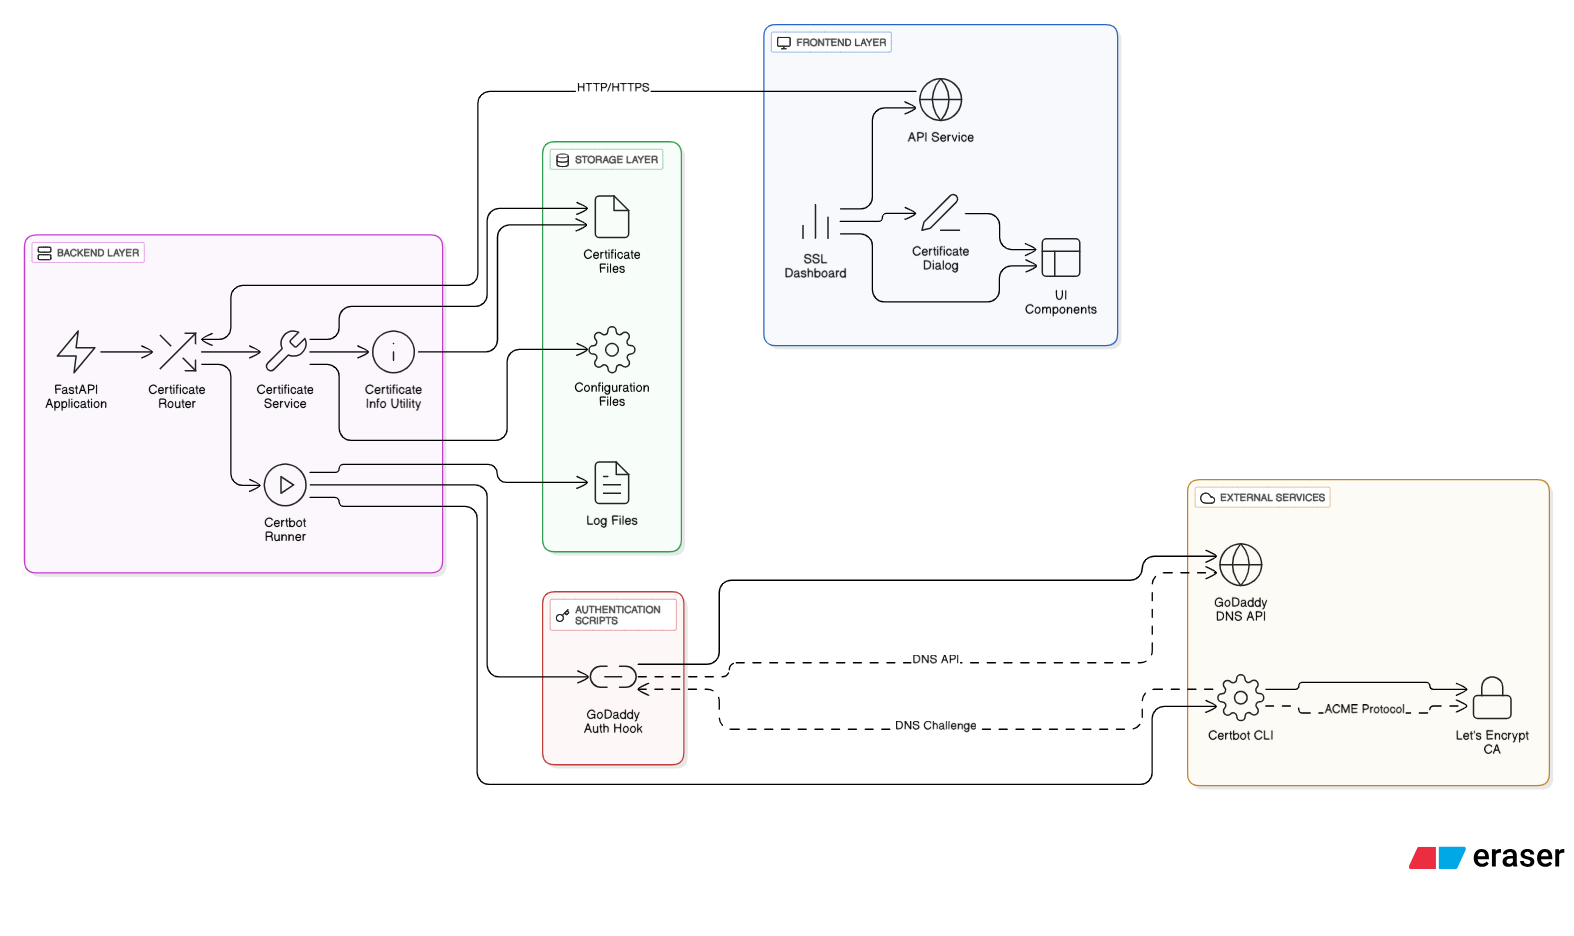
\includegraphics[width=0.9\textwidth]{diagram-images/3.4-component-diagram.png}
\caption{System Component Architecture}
\label{fig:detailed-component-diagram}
\end{figure}

\subsection{System Context}

The system operates within the following context:
\begin{itemize}
    \item Integration with Let's Encrypt Certificate Authority for SSL certificate issuance
    \item Integration with DNS provider APIs (GoDaddy) for domain validation
    \item User interaction through modern web browser interfaces
    \item Containerized deployment on server infrastructure
\end{itemize}

\section{Activity Diagram}

The activity diagram illustrates the workflow of SSL certificate generation process, showing the sequence of activities from user initiation to certificate delivery.

\begin{figure}[h]
\centering
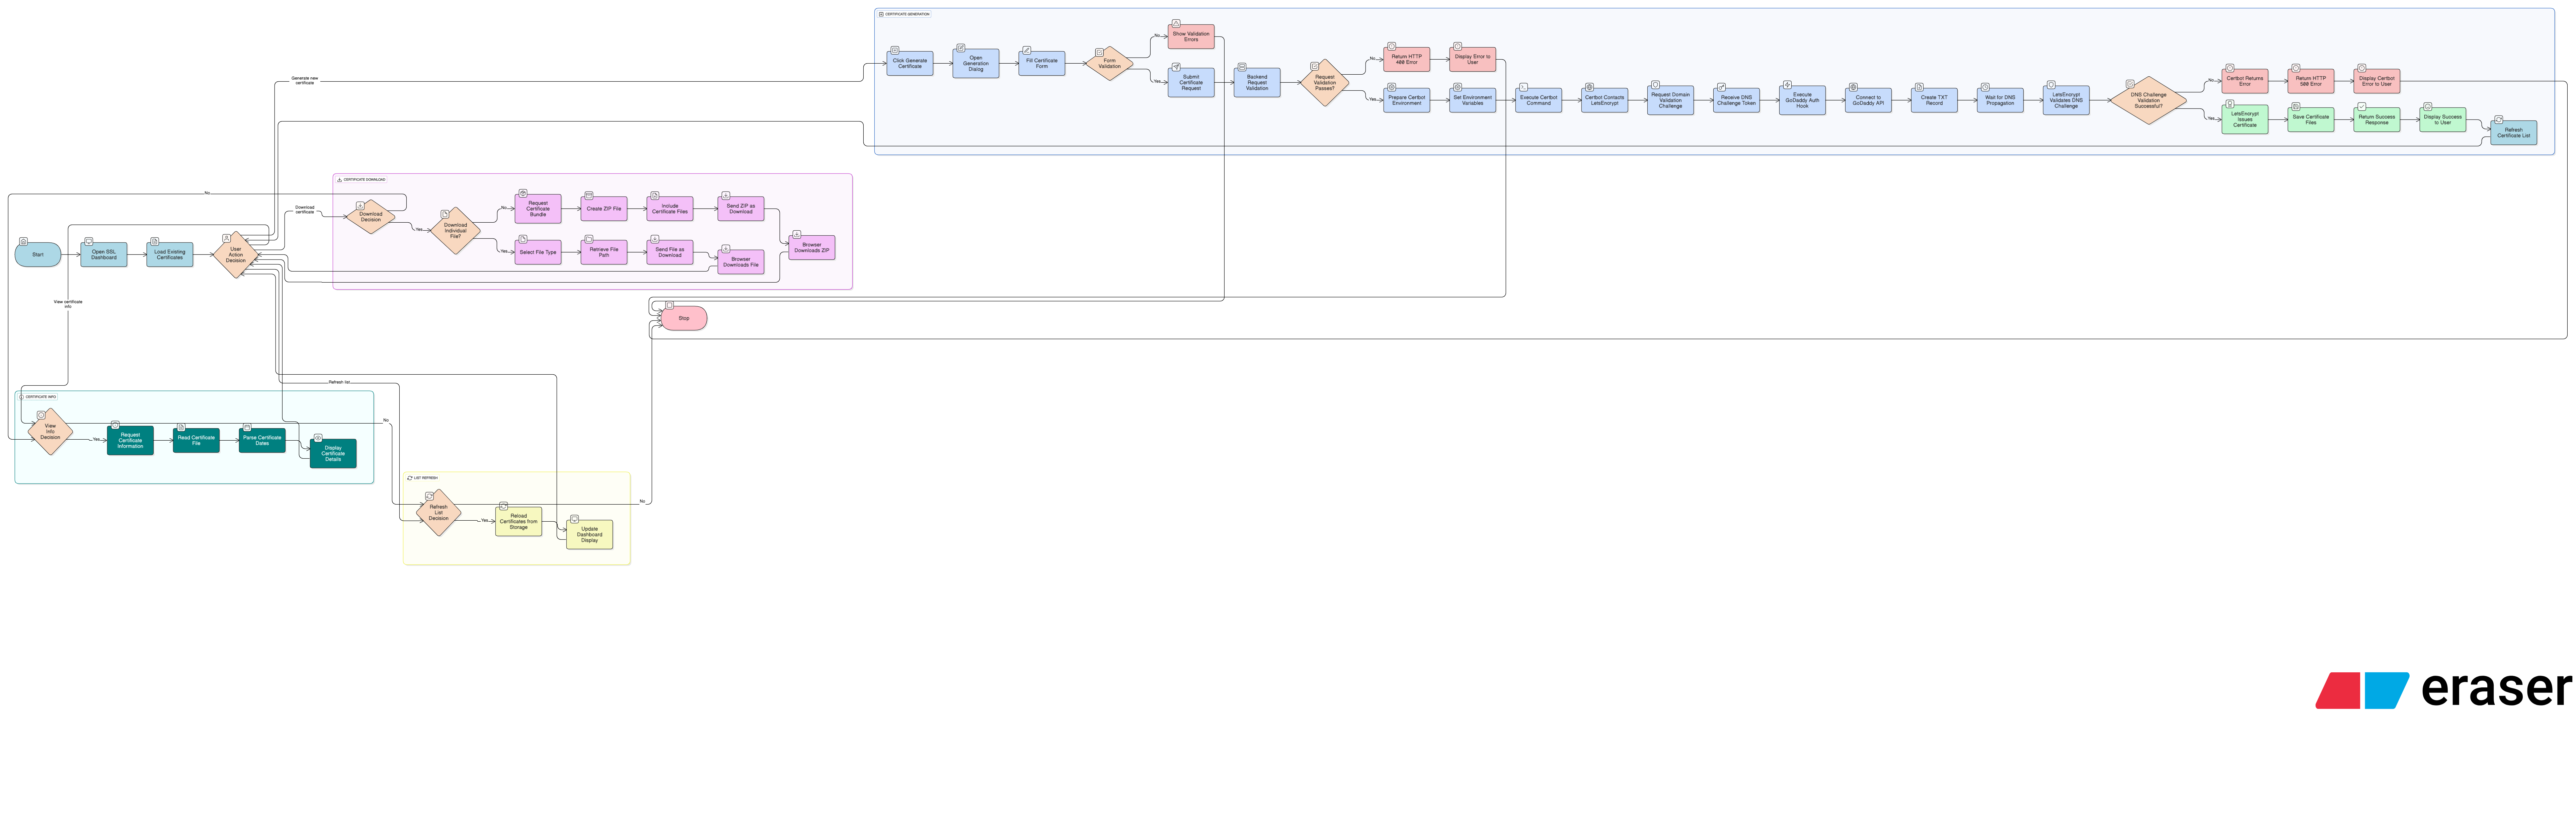
\includegraphics[width=0.8\textwidth]{diagram-images/3.2-activity-diagram.png}
\caption{SSL Certificate Generation Activity Diagram}
\label{fig:activity-diagram}
\end{figure}

The certificate generation process involves the following key activities:
\begin{enumerate}
    \item User provides domain and DNS provider credentials
    \item System validates input parameters and credentials
    \item Certbot initiates ACME challenge with Let's Encrypt
    \item DNS hook script creates TXT record via provider API
    \item Let's Encrypt validates domain ownership
    \item Certificate files are generated and stored
    \item User receives confirmation and download links
\end{enumerate}

\section{Use Case Diagrams}

The use case diagram shows the functional requirements of the system from the user's perspective, identifying the main actors and their interactions with the system.

\begin{figure}[h]
\centering
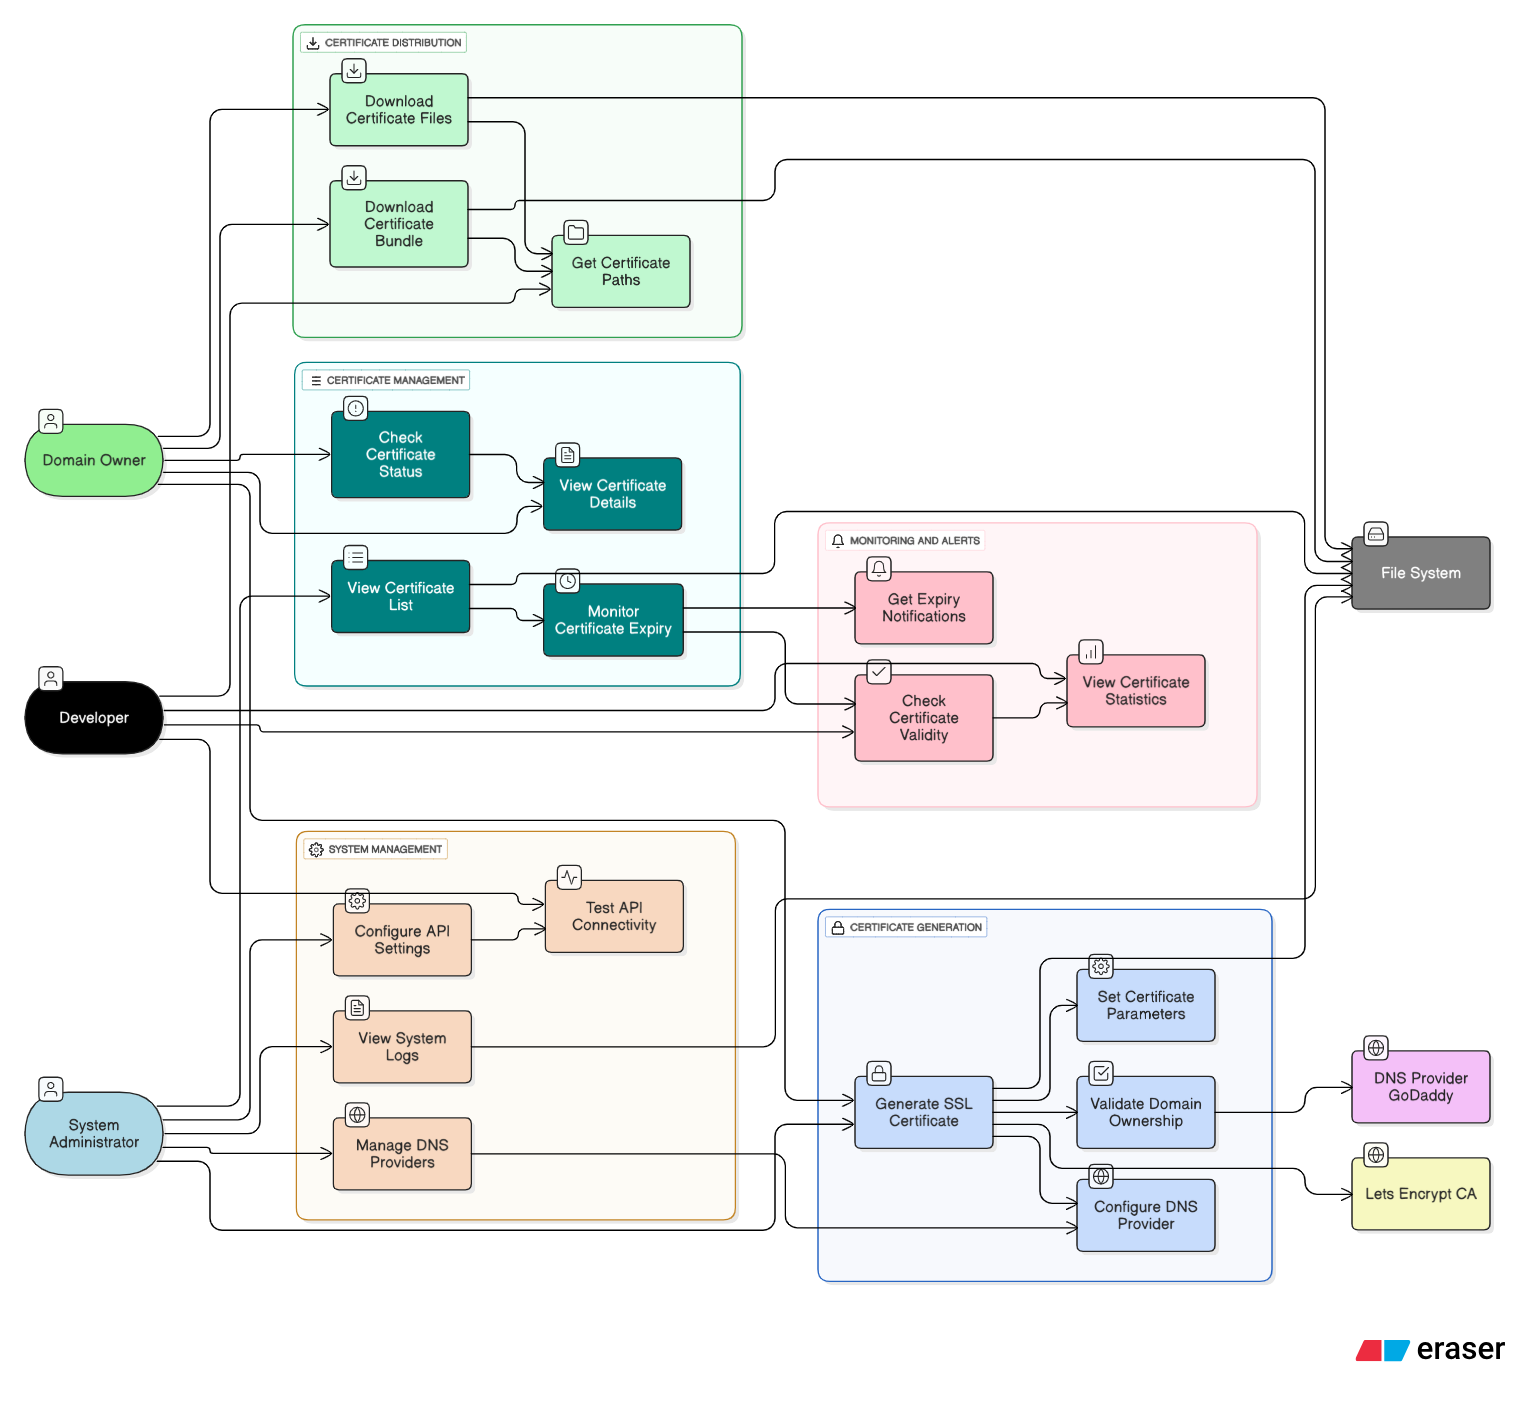
\includegraphics[width=0.9\textwidth]{diagram-images/3.3-use-case-diagram.png}
\caption{SSL Automation Tool Use Case Diagram}
\label{fig:use-case-diagram}
\end{figure}

\subsection{Primary Use Cases}

\begin{enumerate}
    \item \textbf{Generate SSL Certificate}: User initiates certificate generation for a domain
    \item \textbf{View Certificate Status}: User monitors certificate validity and expiration
    \item \textbf{Download Certificate}: User downloads certificate files for deployment
    \item \textbf{Manage DNS Settings}: User configures DNS provider credentials
    \item \textbf{View Documentation}: User accesses server configuration guides
\end{enumerate}

\subsection{Secondary Use Cases}

\begin{enumerate}
    \item \textbf{List All Certificates}: User views comprehensive certificate inventory
    \item \textbf{Download Certificate Bundle}: User downloads ZIP archive of certificate files
    \item \textbf{Check Certificate Info}: User views detailed certificate metadata
    \item \textbf{Configure Advanced Settings}: User adjusts TTL and propagation settings
\end{enumerate}

\section{Component Diagram}

The component diagram shows the high-level software components and their relationships within the SSL Automation Tool architecture.

\begin{figure}[h]
\centering
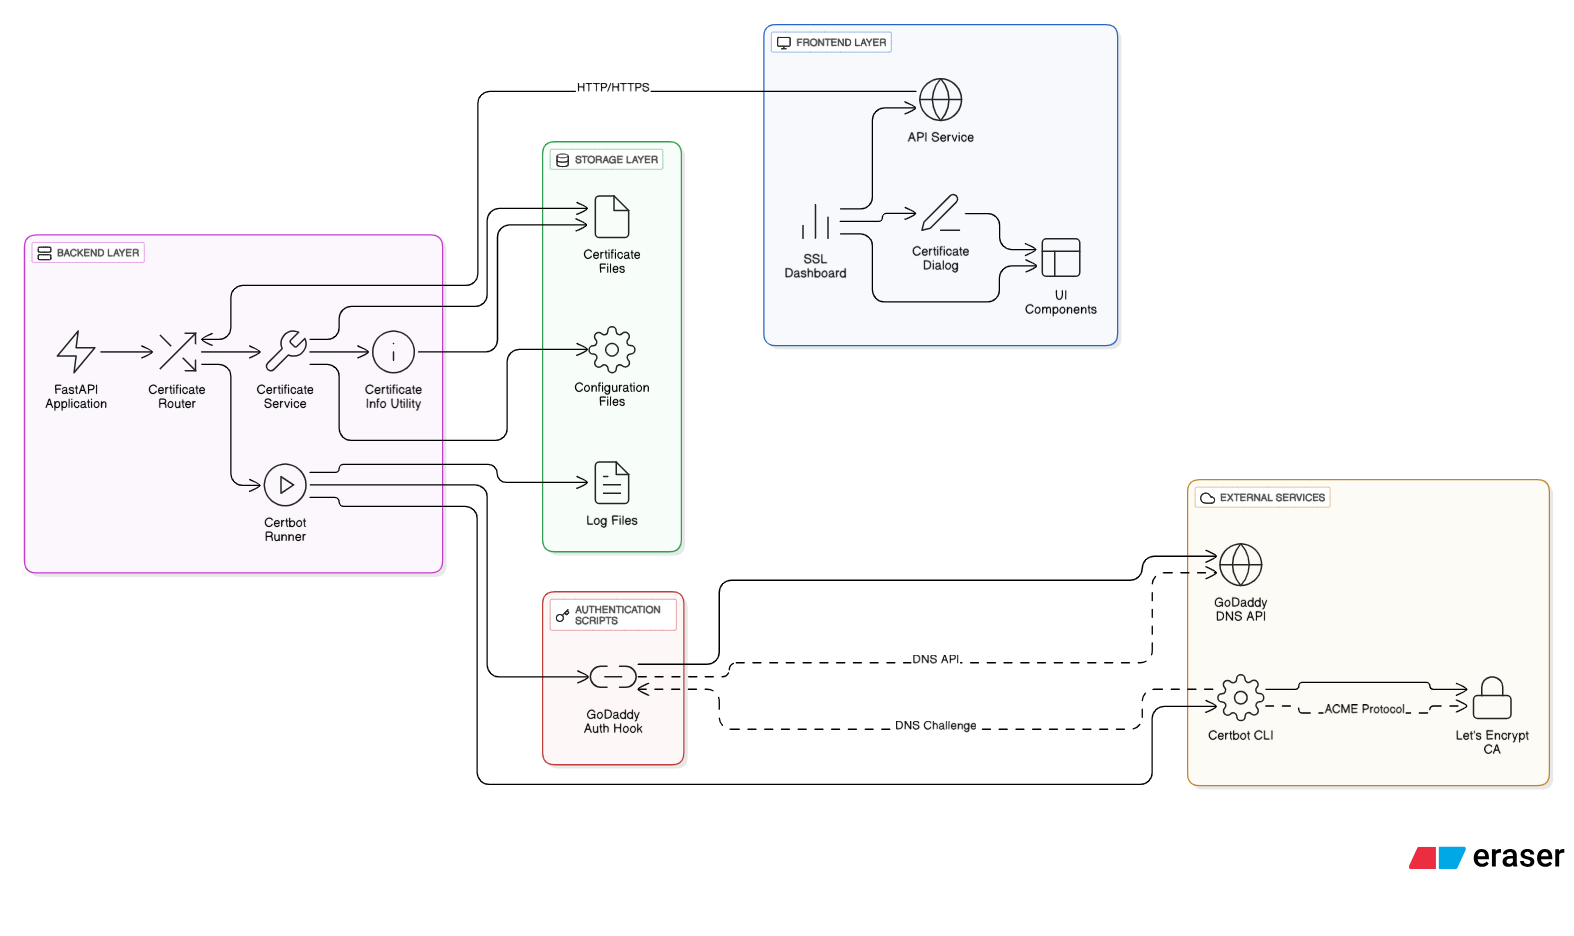
\includegraphics[width=0.9\textwidth]{diagram-images/3.4-component-diagram.png}
\caption{System Component Architecture}
\label{fig:component-diagram}
\end{figure}

\subsection{Frontend Components}

\begin{itemize}
    \item \textbf{React Application}: Main user interface component
    \item \textbf{SSL Dashboard}: Certificate management interface
    \item \textbf{Certificate Forms}: Data input and validation components
    \item \textbf{Documentation System}: Server configuration guides
    \item \textbf{API Service Layer}: HTTP client for backend communication
\end{itemize}

\subsection{Backend Components}

\begin{itemize}
    \item \textbf{FastAPI Application}: REST API server
    \item \textbf{Certificate Service}: Business logic for certificate operations
    \item \textbf{Certbot Runner}: Let's Encrypt integration service
    \item \textbf{DNS Hook Scripts}: DNS provider automation components
    \item \textbf{File Management}: Certificate storage and retrieval
\end{itemize}

\section{Deployment Diagram}

The deployment diagram illustrates the physical architecture and runtime environment of the SSL Automation Tool system.

\begin{figure}[h]
\centering
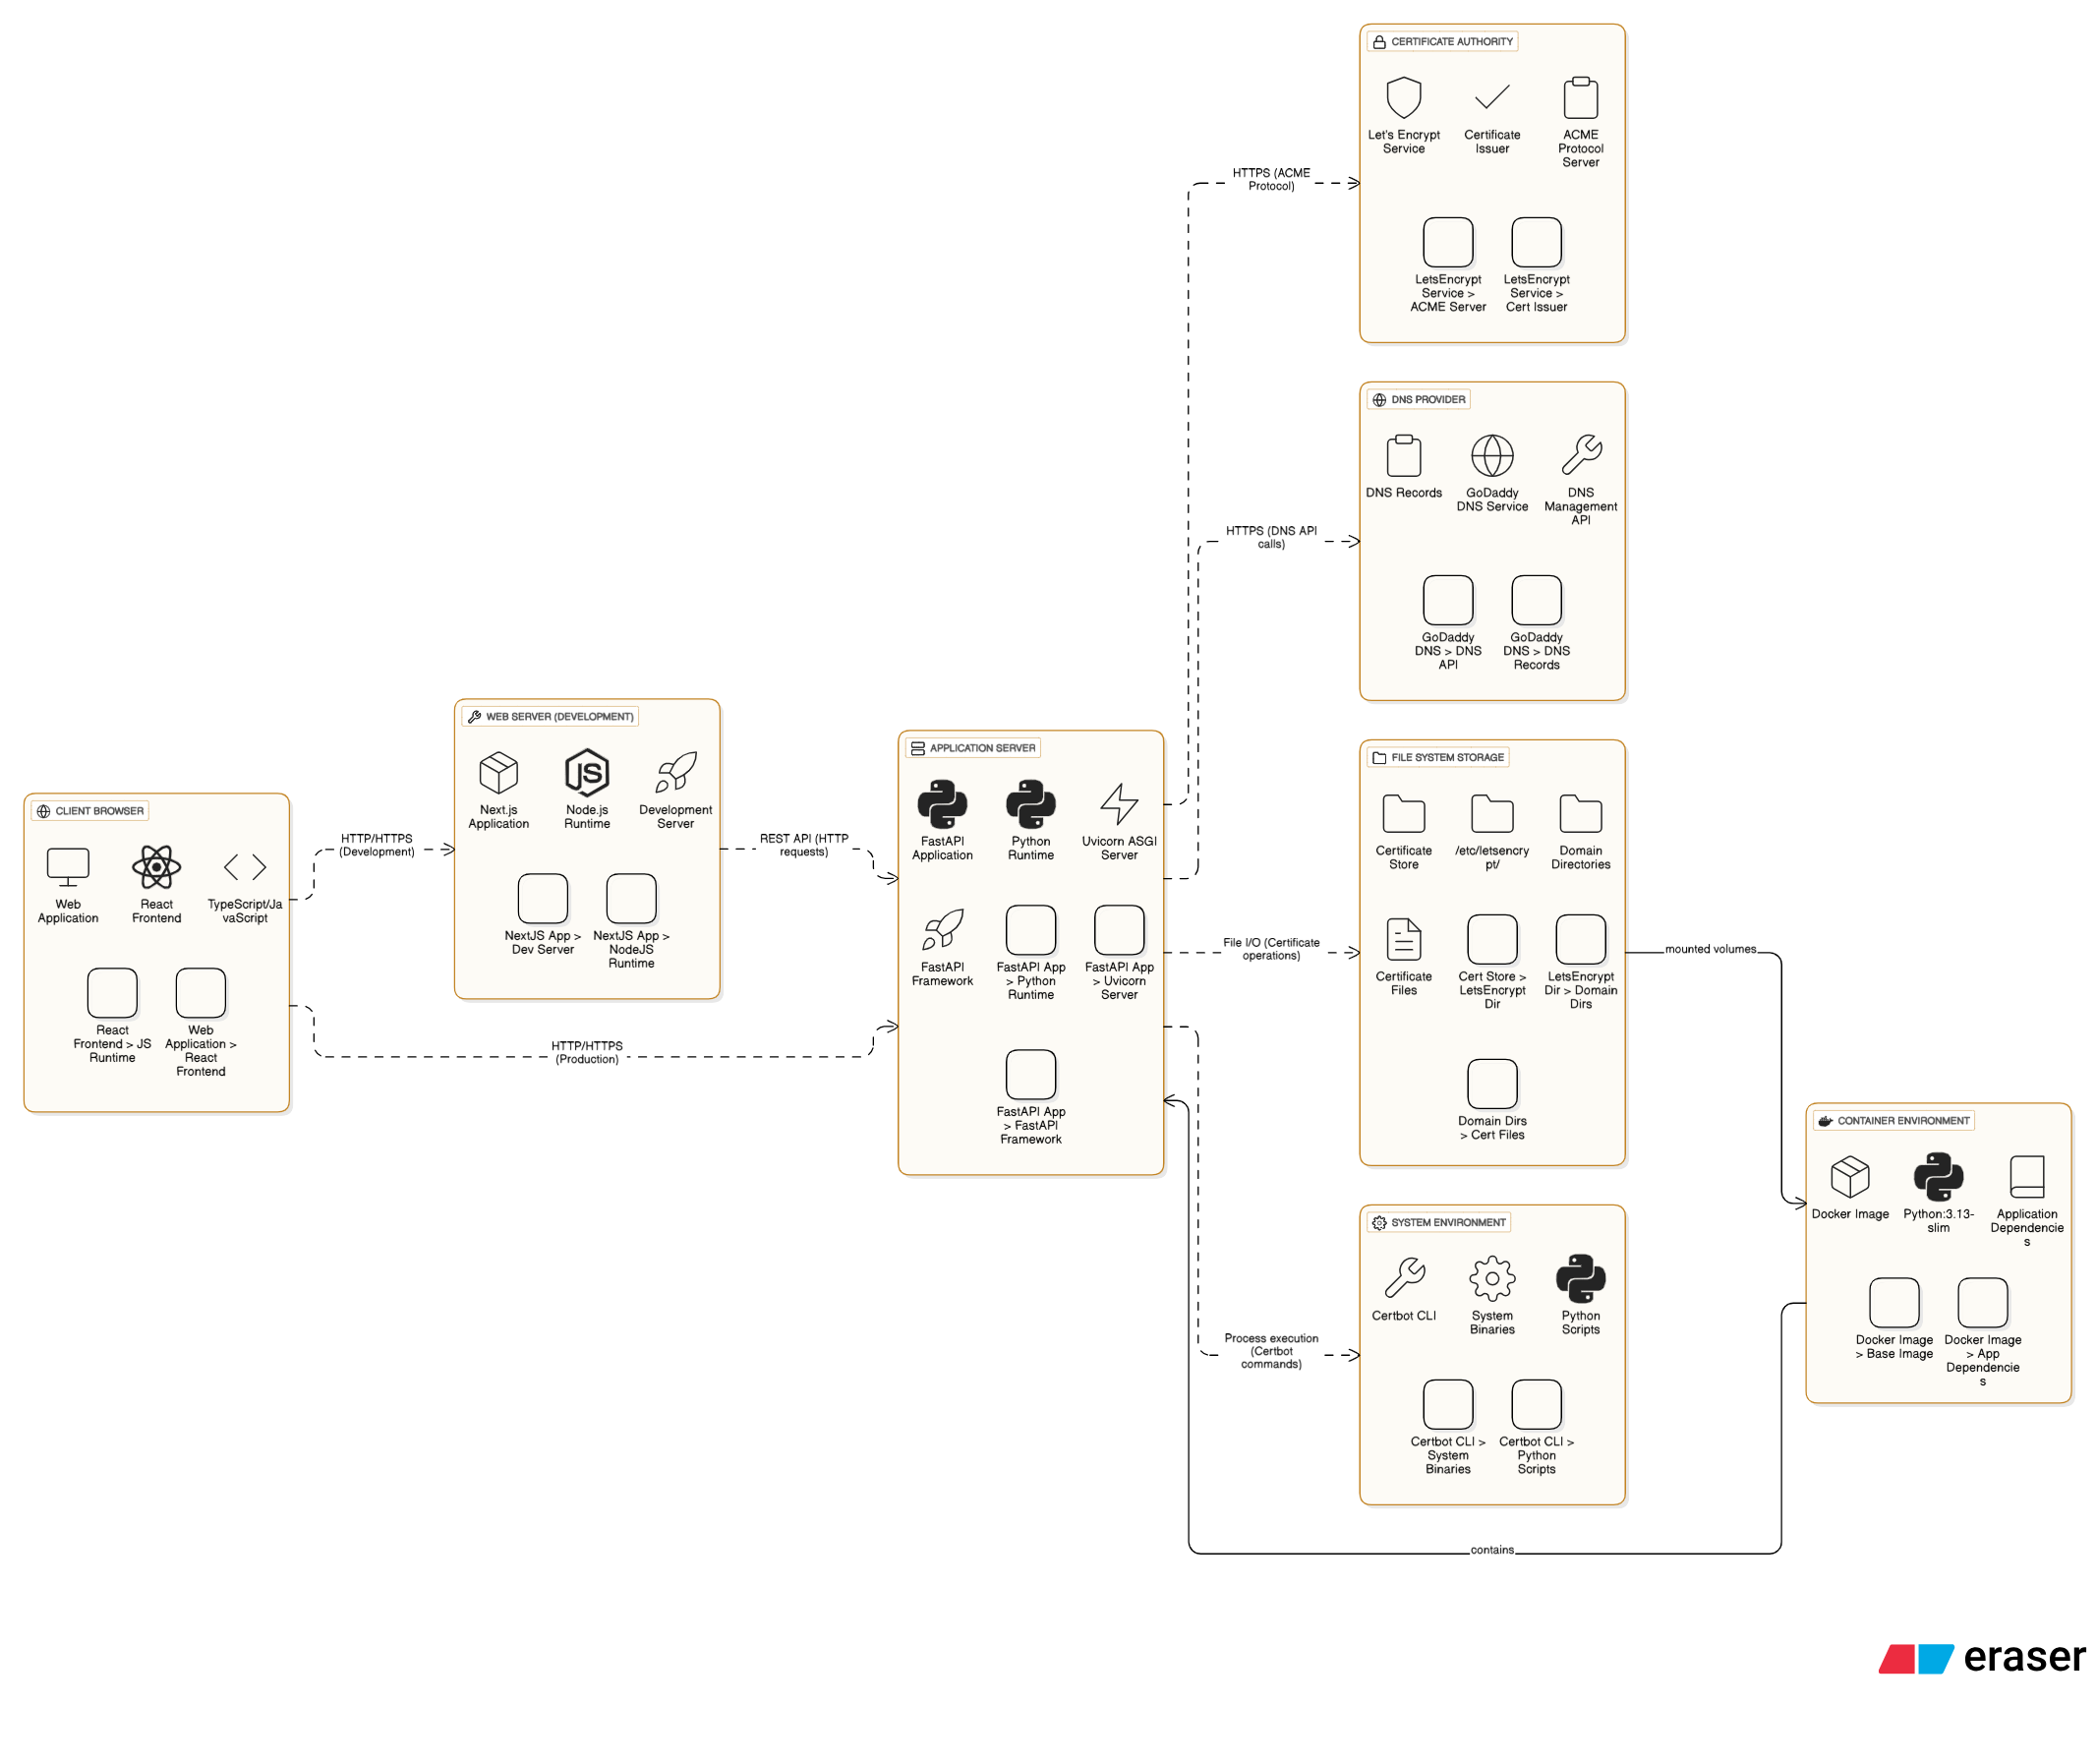
\includegraphics[width=0.9\textwidth]{diagram-images/3.5-deployment-diagram.png}
\caption{System Deployment Architecture}
\label{fig:deployment-diagram}
\end{figure}

\subsection{Deployment Architecture}

\begin{itemize}
    \item \textbf{Client Browser}: User interface execution environment
    \item \textbf{Docker Container}: Application runtime environment
    \item \textbf{Host Server}: Physical or virtual server infrastructure
    \item \textbf{Volume Storage}: Persistent certificate file storage
    \item \textbf{External APIs}: Let's Encrypt and DNS provider services
\end{itemize}

\section{Data Flow Diagram}

The data flow diagram shows how data moves through the system during certificate generation and management operations.

\begin{figure}[h]
\centering
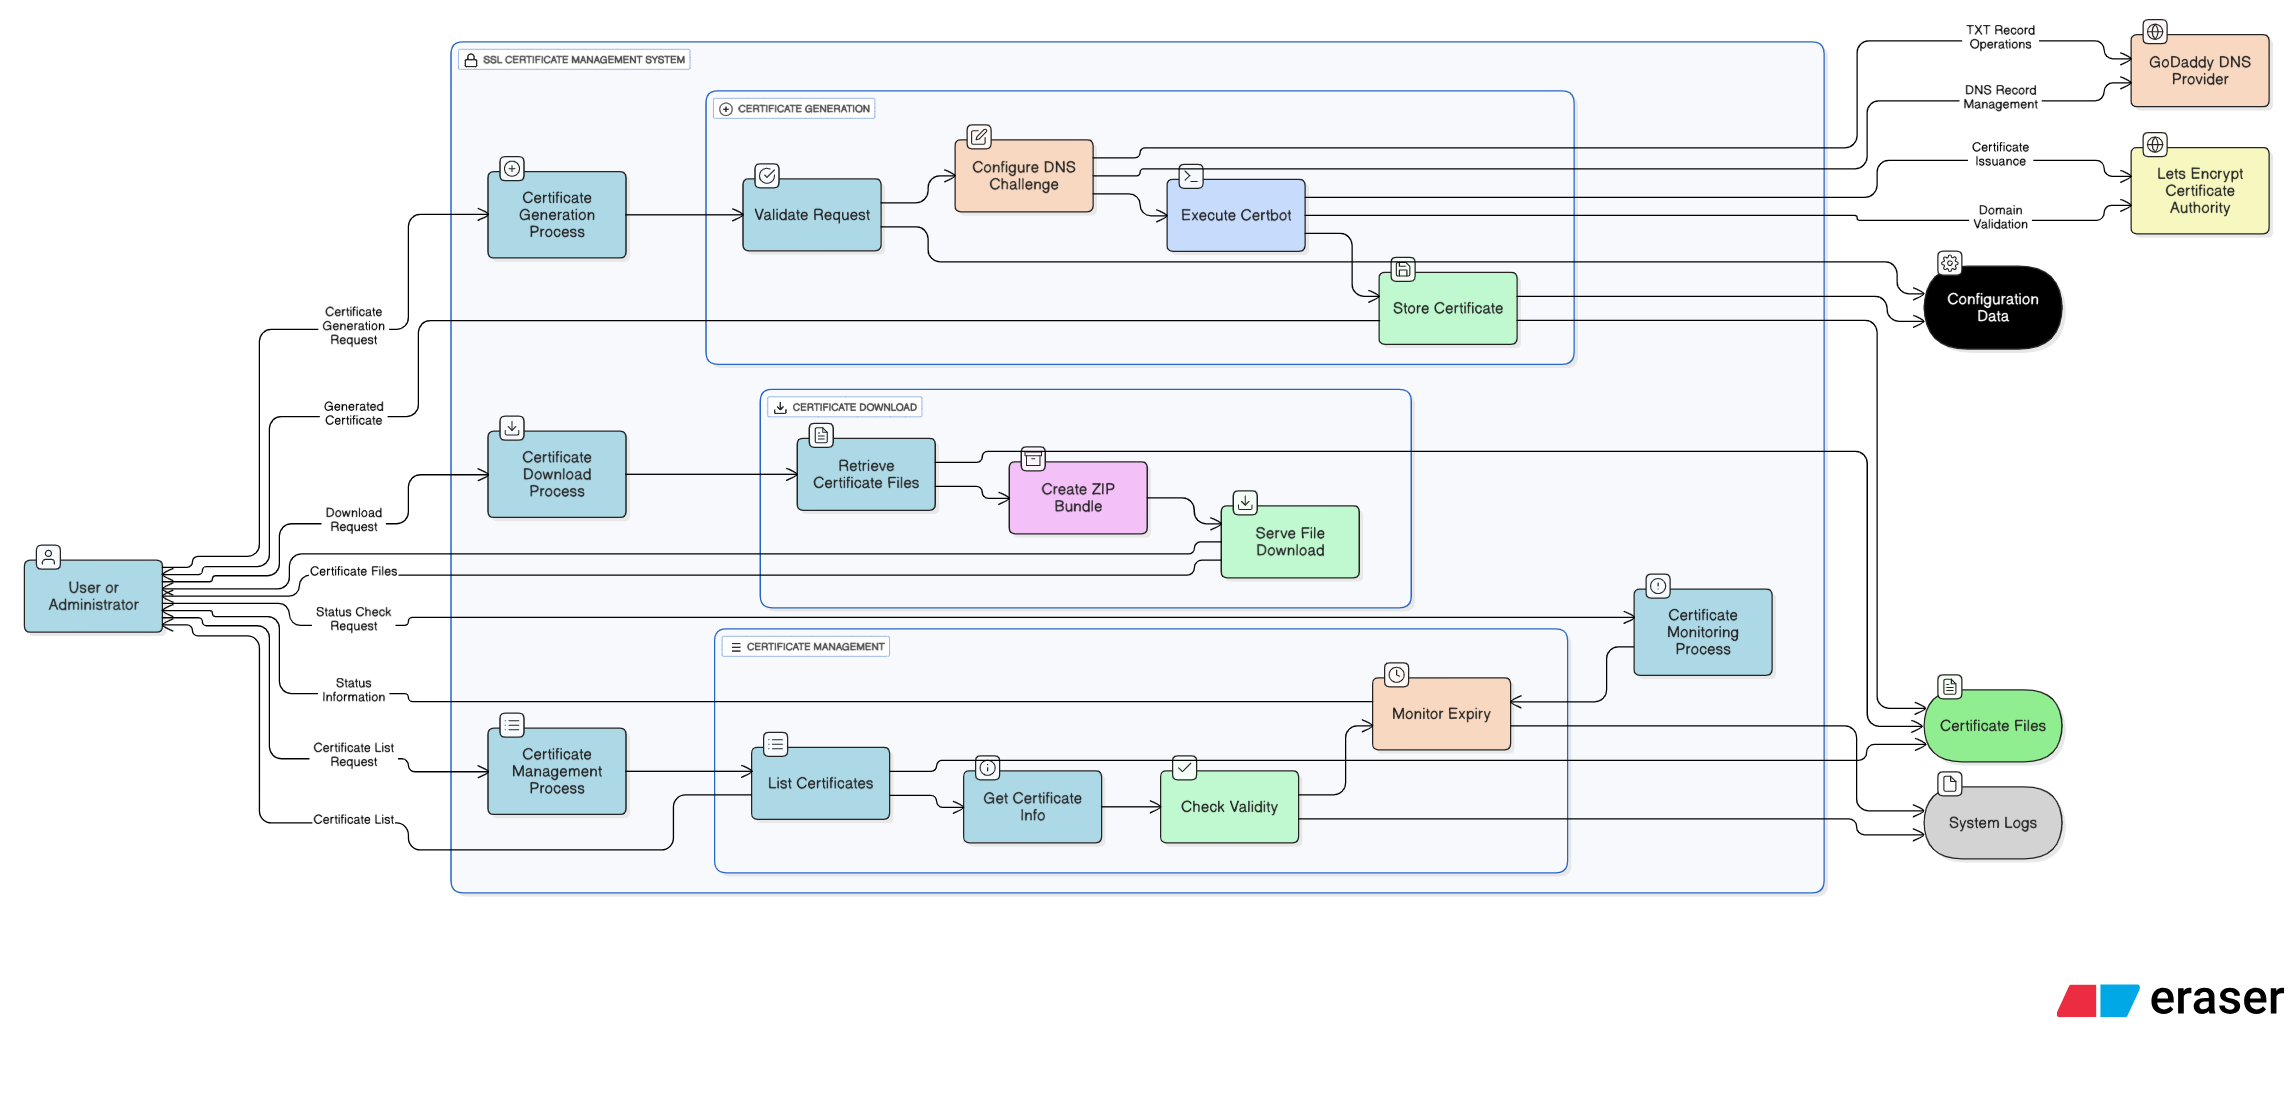
\includegraphics[width=0.9\textwidth]{diagram-images/3.8-data-flow-diagram.png}
\caption{SSL Certificate Data Flow Diagram}
\label{fig:data-flow-diagram}
\end{figure}

\subsection{Data Flow Process}

\begin{enumerate}
    \item User submits certificate request with domain and credentials
    \item Frontend validates and sends request to backend API
    \item Backend initiates Certbot process with challenge data
    \item DNS hook script creates TXT record via provider API
    \item Let's Encrypt validates domain and issues certificate
    \item Certificate files are stored in persistent volume
    \item Certificate metadata is returned to user interface
\end{enumerate}

\section{Functional Decomposition}

The functional decomposition diagram breaks down the system functionality into hierarchical components showing the relationship between different system functions.

\begin{figure}[h]
\centering
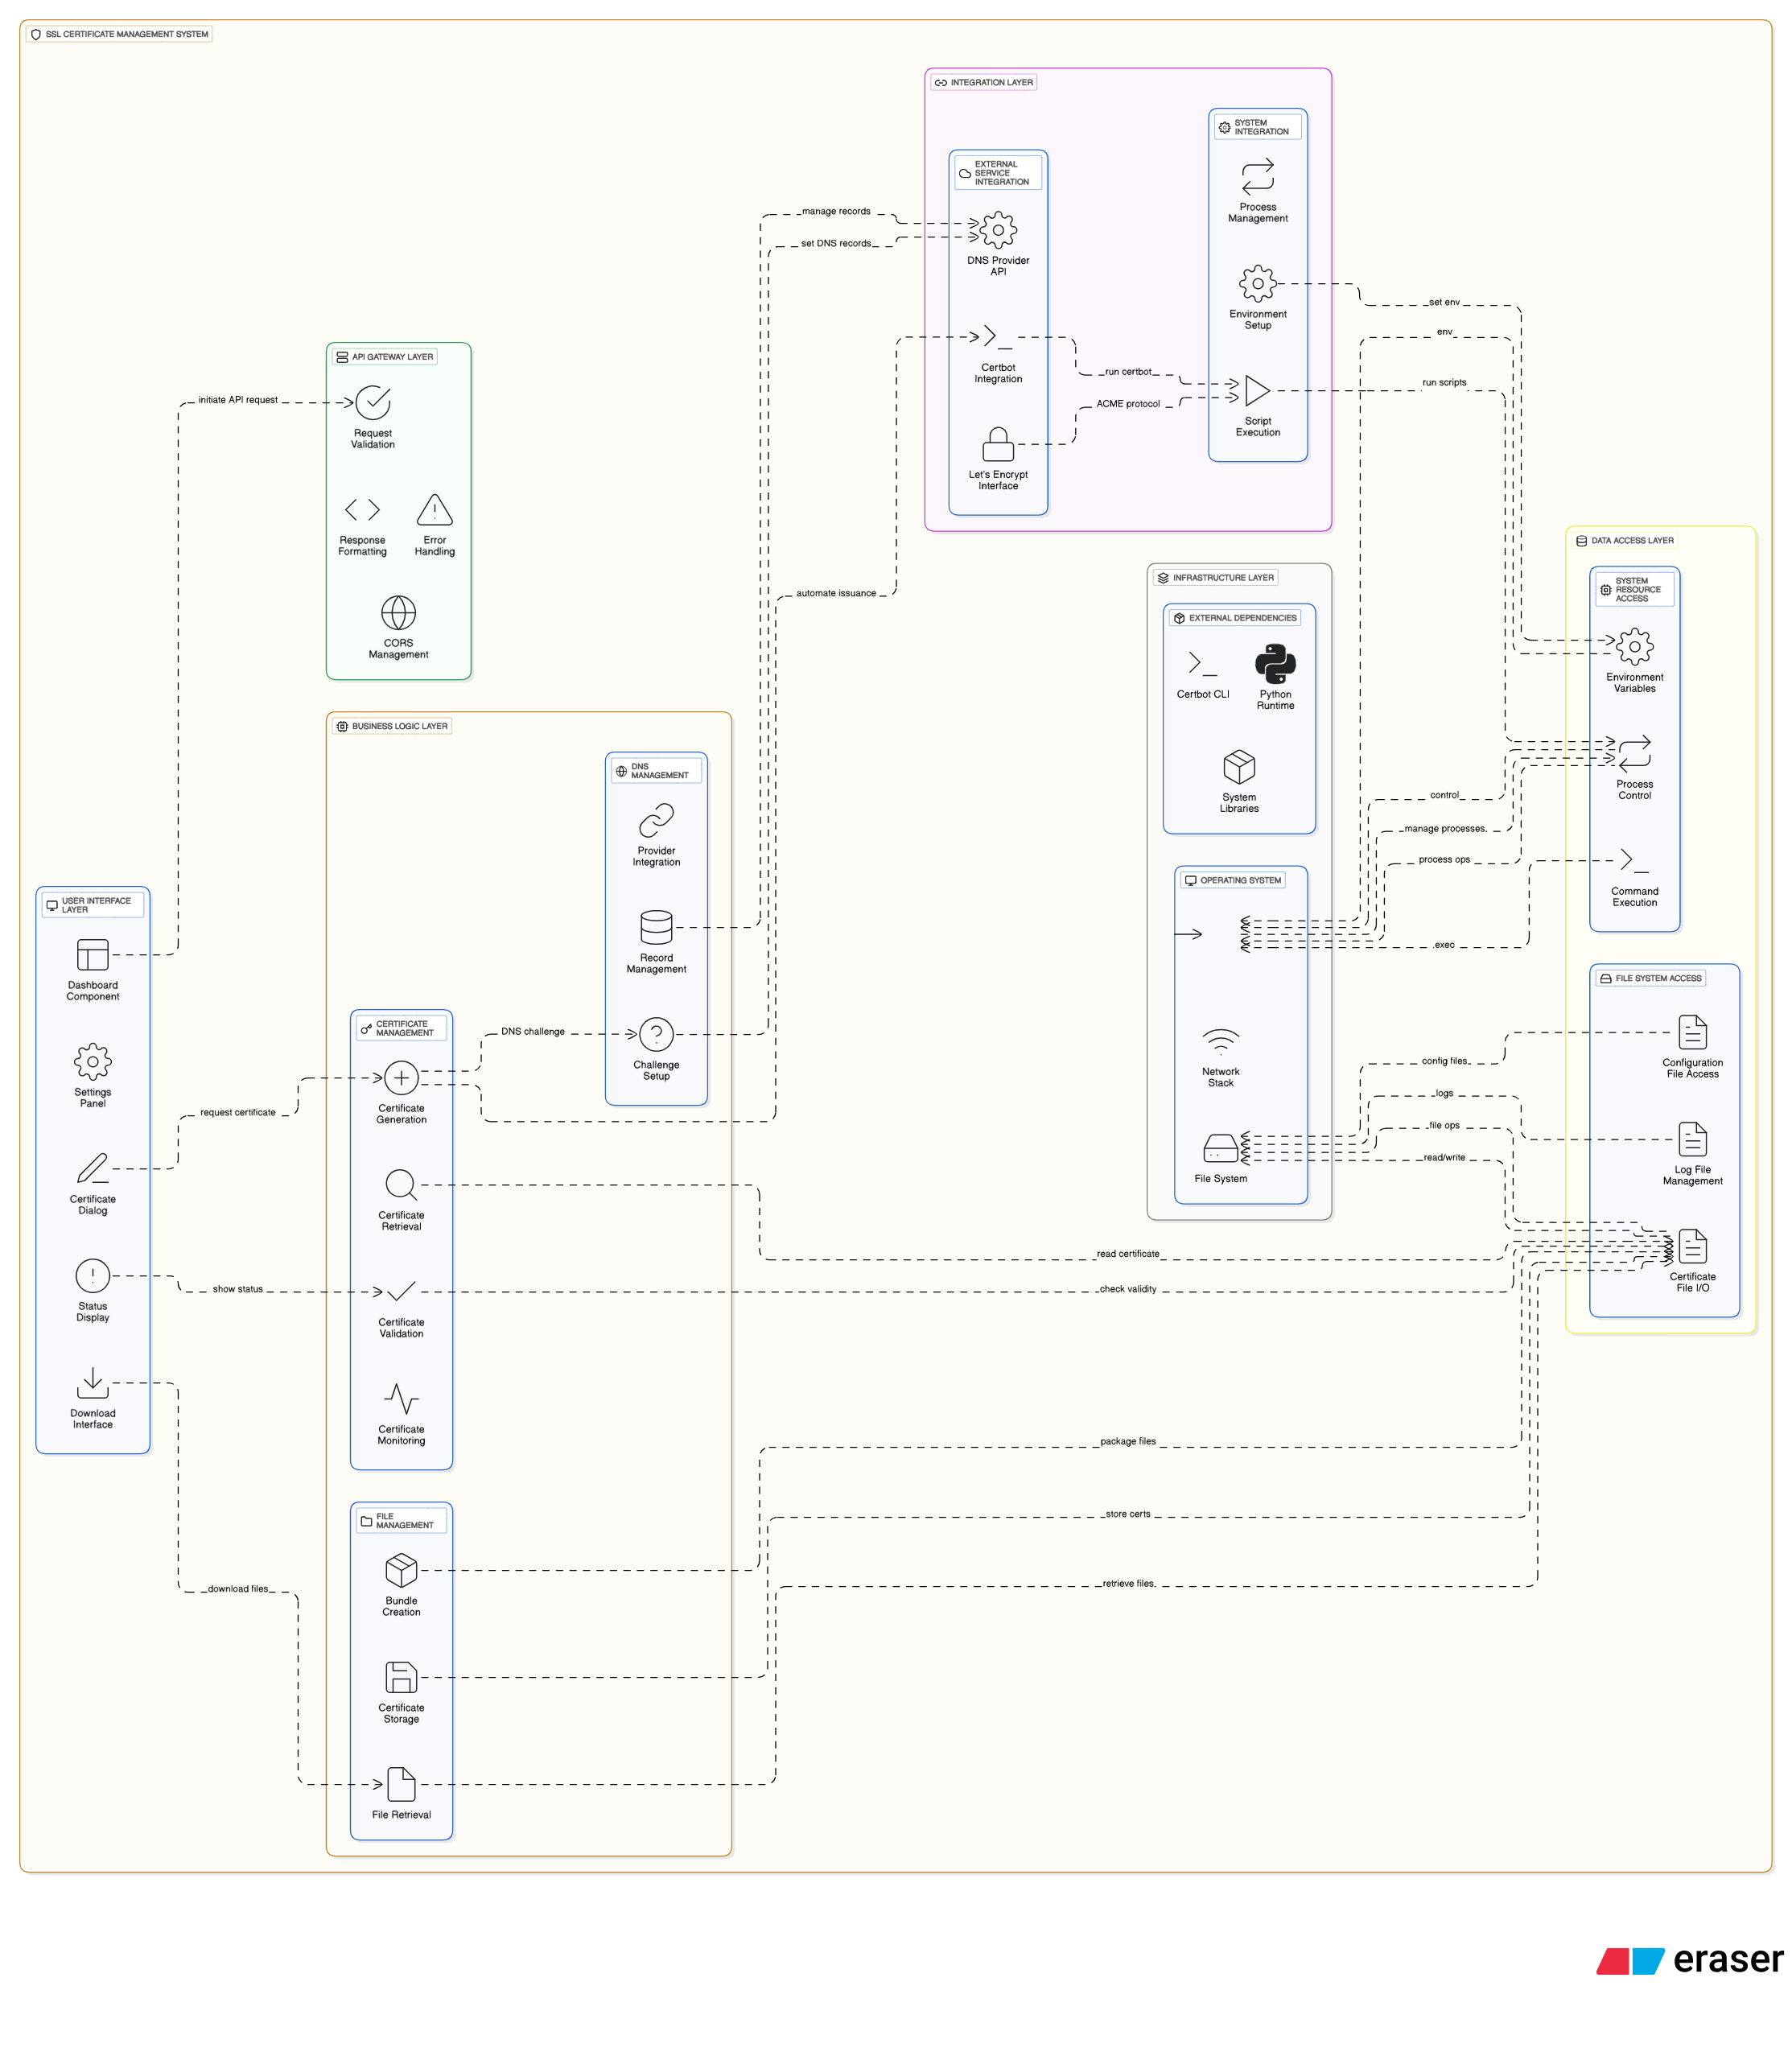
\includegraphics[width=0.9\textwidth]{diagram-images/3.9-functional-decomposition.png}
\caption{Functional Decomposition Diagram}
\label{fig:functional-decomposition}
\end{figure}

\subsection{Function Hierarchy}

\begin{itemize}
    \item \textbf{Certificate Management}
    \begin{itemize}
        \item Certificate Generation
        \item Certificate Validation
        \item Certificate Storage
        \item Certificate Retrieval
    \end{itemize}
    
    \item \textbf{DNS Operations}
    \begin{itemize}
        \item Provider Authentication
        \item TXT Record Management
        \item Domain Validation
        \item Propagation Handling
    \end{itemize}
    
    \item \textbf{User Interface}
    \begin{itemize}
        \item Form Management
        \item Status Monitoring
        \item File Downloads
        \item Documentation Display
    \end{itemize}
\end{itemize}

\section{Test Procedures and Implementation}

The testing strategy ensures system reliability and functionality through comprehensive test coverage.

\begin{figure}[h]
\centering
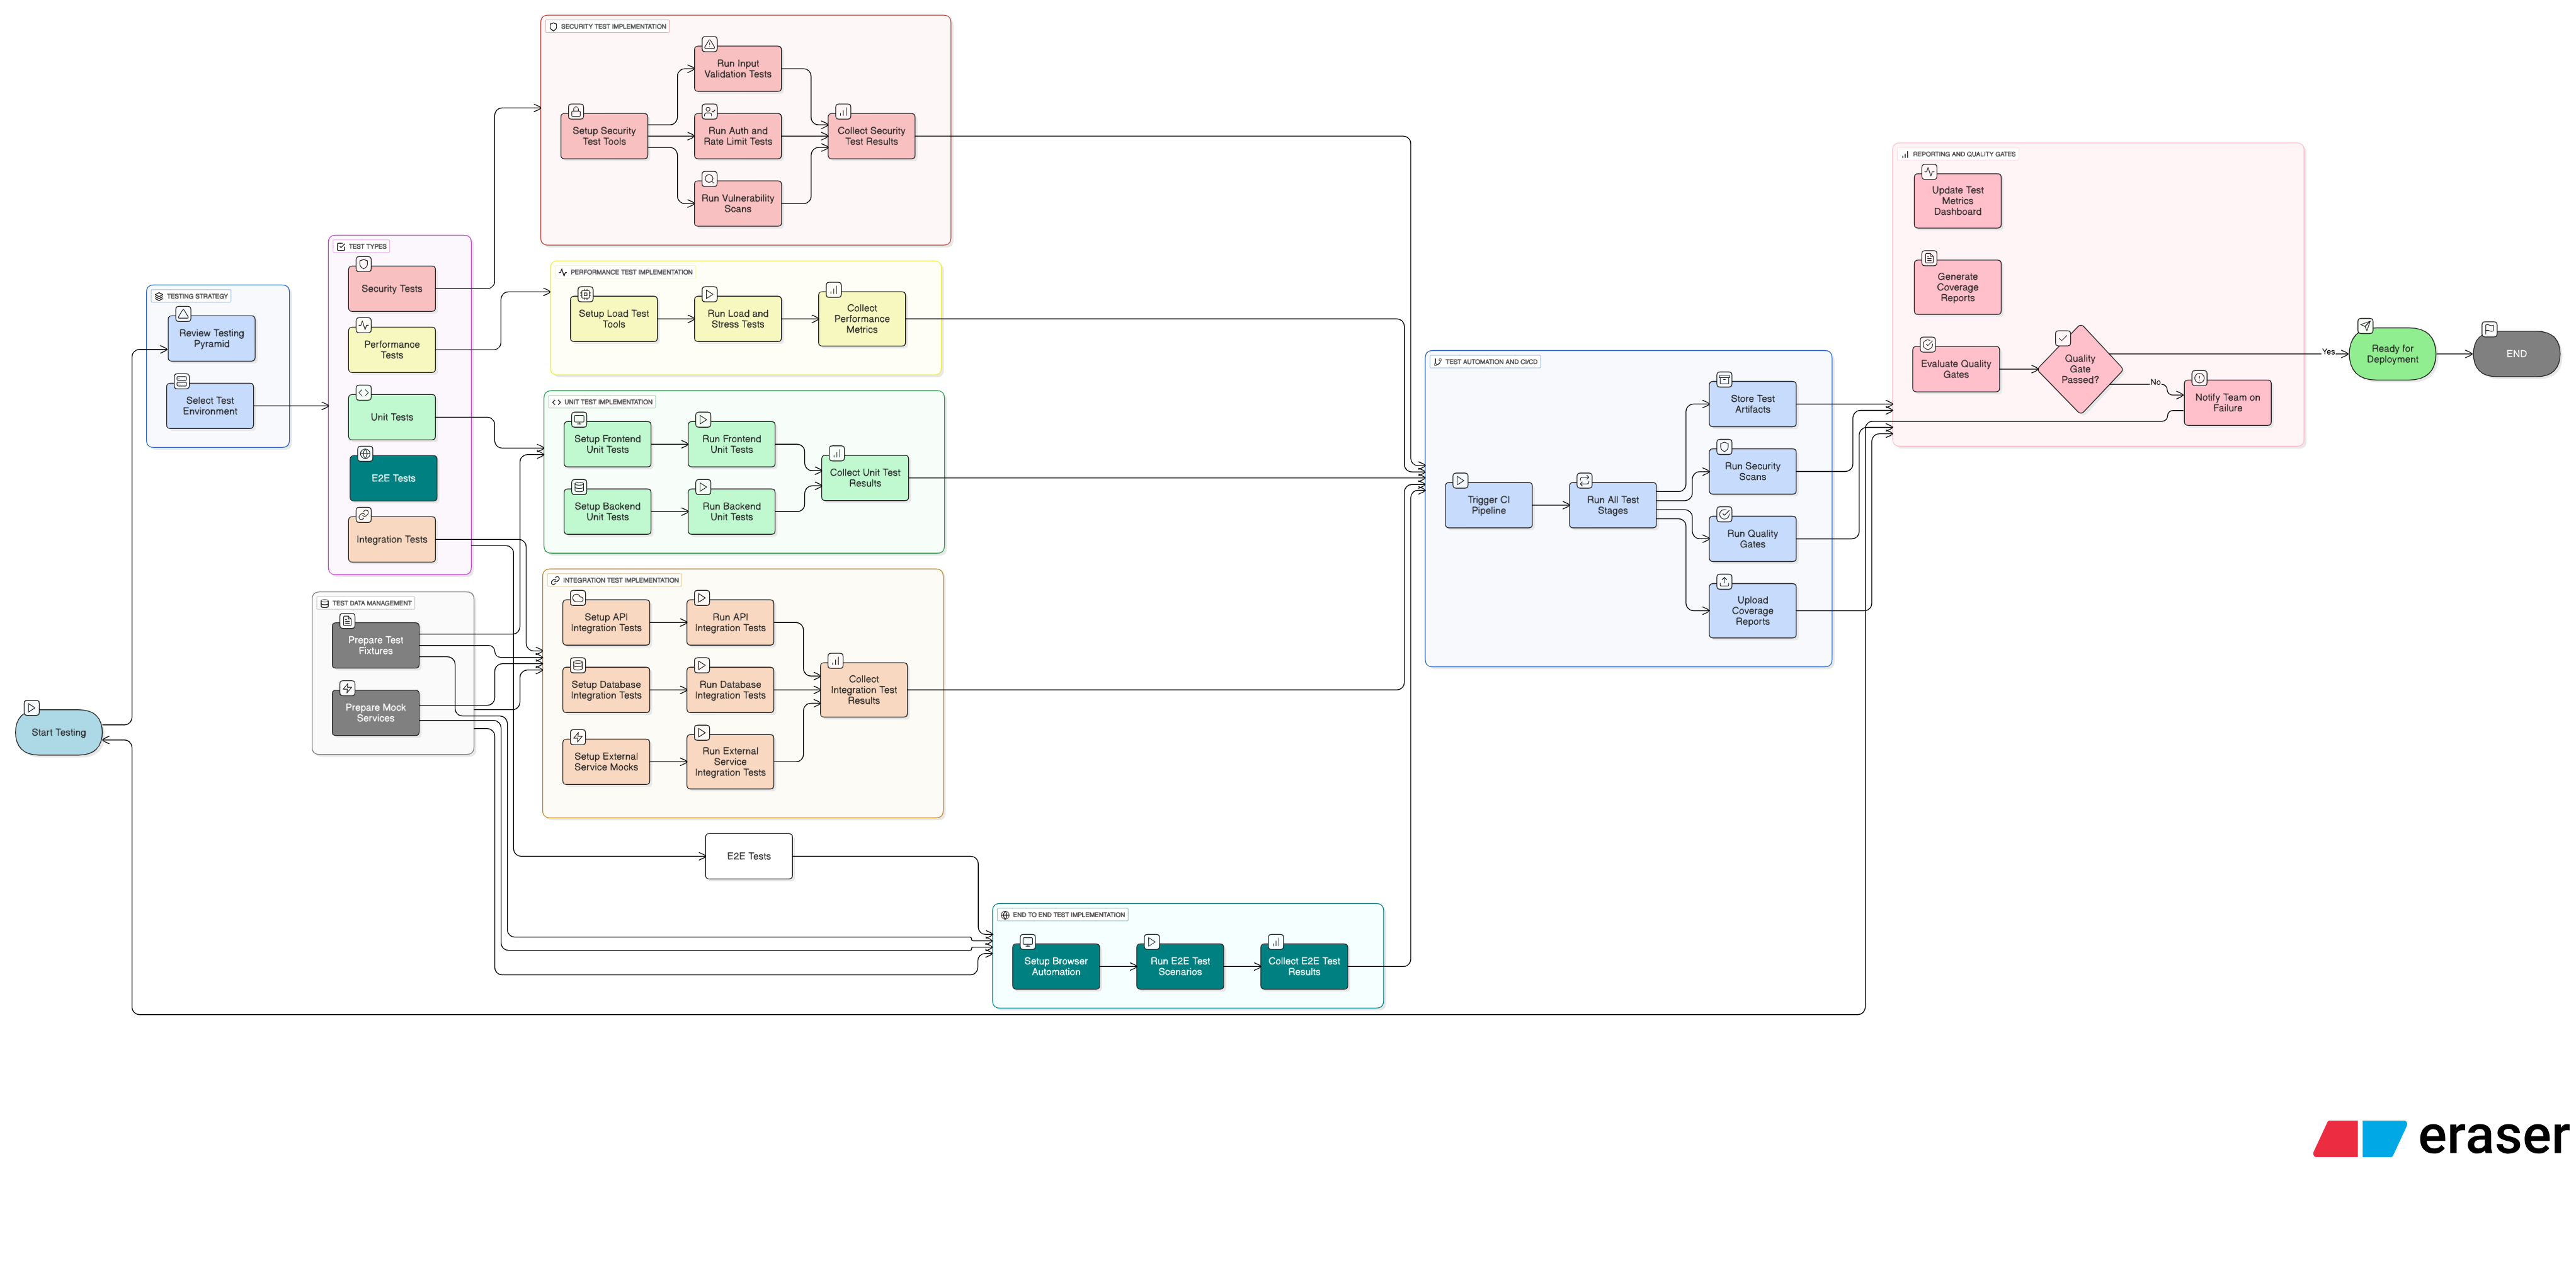
\includegraphics[width=0.9\textwidth]{diagram-images/3.16-test-procedures.png}
\caption{Test Procedures and Implementation}
\label{fig:test-procedures}
\end{figure}

\subsection{Testing Levels}

\begin{enumerate}
    \item \textbf{Unit Testing}
    \begin{itemize}
        \item Individual component functionality testing
        \item API endpoint validation
        \item DNS integration testing
        \item Certificate parsing validation
    \end{itemize}
    
    \item \textbf{Integration Testing}
    \begin{itemize}
        \item Frontend-backend communication testing
        \item Let's Encrypt ACME protocol integration
        \item DNS provider API integration
        \item End-to-end certificate generation workflow
    \end{itemize}
    
    \item \textbf{System Testing}
    \begin{itemize}
        \item Complete system functionality validation
        \item Performance testing under load
        \item Security testing for credential handling
        \item Browser compatibility testing
    \end{itemize}
    
    \item \textbf{User Acceptance Testing}
    \begin{itemize}
        \item User interface usability testing
        \item Documentation completeness validation
        \item Real-world scenario testing
        \item Error handling verification
    \end{itemize}
\end{enumerate}

\subsection{Test Implementation Strategy}

\begin{itemize}
    \item \textbf{Automated Testing}: Unit tests for utility functions and API endpoints
    \item \textbf{Manual Testing}: User interface and integration scenarios
    \item \textbf{Staging Environment}: Let's Encrypt staging server for safe testing
    \item \textbf{Continuous Integration}: Automated test execution on code changes
\end{itemize}